\chapter{Apêndices}

\section{Sistemas de Tempo Real}
São sistemas computacionais que dependem não somente da correção dos dados computados, mas que sejam obtidos dentro de um intervalo 
de tempo 
pré determinado, que pode ser maior ou menor de acordo com a aplicação.
Na literatura, este período em que se espera que a resposta do sistema se dê é denominado \textit{deadline}.
Sistemas de tempo real podem ser classificados em dois tipos: \textit{soft} ou \textit{hard}.

Sistemas \textit{soft} são menos restritivos, tolerando eventuais perdas de \textit{deadline}; 
ao contrário dos sistemas \textit{hard}, em que estas perdas não são aceitáveis.  

Algumas características típicas, apesar de não obrigatórias, de sistemas de tempo real são limitações com relação ao tamanho, propósito específico e 
baixo custo \cite{silberschatz}.

\section{CRC}
Método de detecção de erros aleatórios, isto é, de dados corrompidos ao longo do processo de transmissão ou armazenamento da informação por exemplo 
por ruídos, mas não por um agente \textquoteleft inteligente\textquoteright{} externo que modifique os dados transmitidos, tal qual um 
\textit{malware} \cite{stigge}.

Consiste essencialmente em uma divisão polinomial \cite{stigge}, logo, pode ser implementado em \textit{hardware}, utilizando-se apenas registradores 
de deslocamento com conexões realimentadas \cite{peterson}, assim como em \textit{software}. 
Em suma, trata-se de acrescentar à mensagem digital original um sufixo, que tem seu valor definido por operações realizadas em função da mensagem 
binária que se intenta enviar e de um polinômio gerador.
Para o \textit{transceiver} nRF24L01+, dois polinômios geradores são utilizados: Eq. \ref{CRC_1} quando o dado cíclico adicionado é de 1 
\textit{byte} , e Eq. \ref{CRC_2}, para 2 \textit{bytes} \cite{nRF}.

Para uma descrição completa de como é implementado este método, vide \citeonline{stigge,peterson}.

\begin{equation}
\label{CRC_1}
G(X) = X^8 + X^2 + X + 1 
\end{equation}

\begin{equation}
\label{CRC_2}
G(X) = X^{16} + X^{12} + X^5 + 1 
\end{equation}

\section{PWM}
A modulação por largura de pulso é uma técnica de modulação que consiste em amostrar e codificar o sinal correspondente à mensagem na largura de um 
trem de pulsos de amplitude fixa, i.e. cada amostra da mensagem é convertida em um pulso retangular cuja duração expressa a amplitude do sinal 
modulante.

Um modulador PWM pode ser implementado utilizando-se um circuito comparador não inversor cuja entrada inversora liga-se à saída de um gerador de 
ondas tipo dente de serra (\textit{trailing edge modulation}), dente de serra invertida (\textit{leading edge modulation}  ou triangular 
(\textit{modulation on both edges}) e na entrada não inversora, o sinal modulante. 
Desta forma, quando a tensão da mensagem excede a amplitude da onda gerada, observa-se um sinal alto na saída, caso contrário, baixo, conforme 
ilustra a Fig. \ref{pwm_modulation_types}.

  \begin{figure}[H] %% TODO fonte: https://en.wikipedia.org/wiki/File:Three_PWM_types.svg
    \centering
    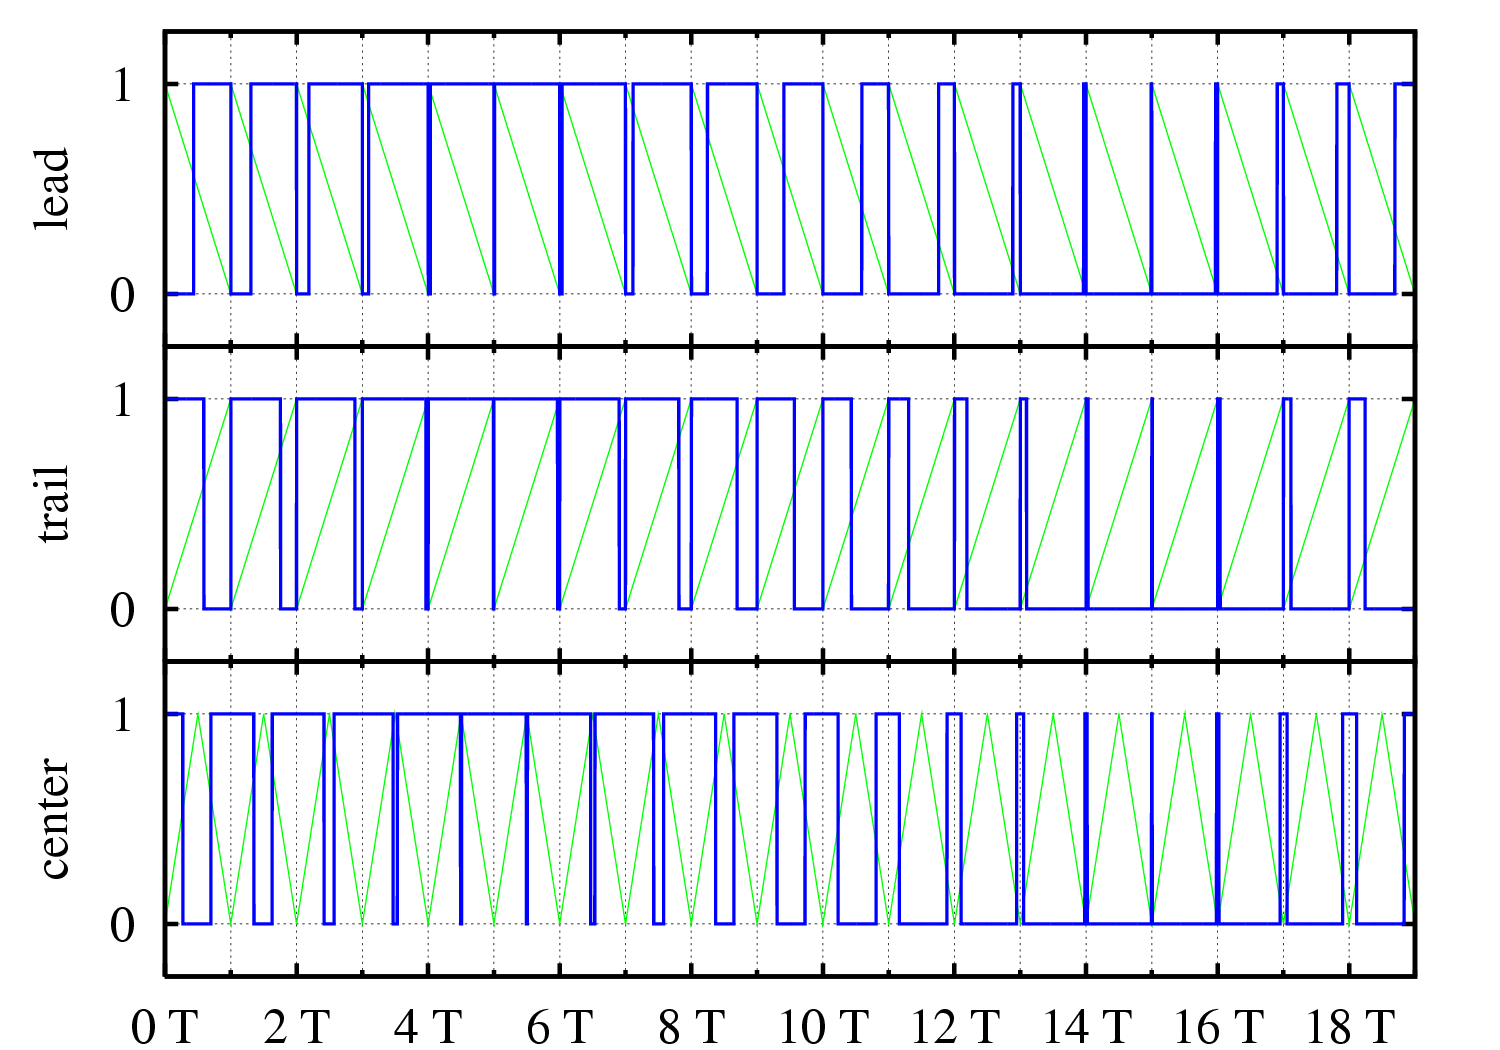
\includegraphics[width=0.7\linewidth]{../../Imagens/PWM_modulation_types.png}
    \caption{Três tipos de modulação PWM: \textit{trailing edge}, \textit{leading edge} e  \textit{both edges}, de cima pra baixo, respectivamente.}
    \label{pwm_modulation_types}
  \end{figure}
  
para uma descrição detalhada do circuito e simulações vide \citeonline{pwm_modulator}
  
  %TODO circuito corretor de erros:
%    First, the error amplifier accommodates feedback of the output PWM waveform in order to correct for any errors in the
% output voltage introduced by the comparator. Second, it adds a dc offset to the input voltage so that negative input voltages can be accommodated 
% by 
% the circuit.
%  
%  Because the supply voltage of the comparator directly impacts the output voltage, PWM circuits without feedback have no power supply rejection. In 
% this TI Design, the error amplifier acts as an inverting amplifier to the input signal, shown as a dc-coupled source VIN. By including the 
% comparator 
% inside the feedback loop of the error amplifier, and adding integration capacitor C1, the error amplifier now directly controls the average output 
% voltage
% 
% 
